\documentclass{article}
\usepackage{amsmath}
\usepackage{amssymb}
\usepackage{parallel}
\usepackage[most]{tcolorbox}
\usepackage{amsthm}
\usepackage{caption}
\usepackage{subcaption}
\usepackage[a4paper,
top=1.5cm,
bottom=1.5cm,
left=1.8cm,
right=1.8cm,
heightrounded]
{geometry}
\renewcommand{\arraystretch}{2.5}

\title{\textbf{QF605 Group Project}}

\author{\textbf{Group Members:} \\ \textbf{Kim Chan-Jung, Jin Weiguo , Johnny Quek,} \\ \textbf{Wang Boyu, Woon Tian Yong}}

\date{}

\begin{document}
	\maketitle
		
	\begin{abstract}
		\noindent \textbf{Part I - Bootstrapping Swap Curves} \\ \\
		
		
		\noindent \textbf{Part II - Swaption Calibration}\\ \\
	
		
		\noindent \textbf{Part III - Convexity Correction}\\ \\		

		
		\noindent \textbf{Part IV - Decompounded Options}\\ 
		
		
	\end{abstract} 
\newpage	
% PART 1: Bootstrappng Swap curves %%%%%%%%%%%%%%%%%%%%%%%%%%%%%%%%%%%%%%%%%%%%%%%%
\section*{Part I: Bootstrapping Swap Curves}
\section{OIS Discount Factors}

\noindent With the provided OIS rates data, we proceeded to use the following methodology to bootstrap the OIS discount factor curve. 

\begin{align*}
PV_{fix} &= PV_{float} \\
D(0,1y) * OIS_{1y} &= D(0,1y) * [ (1 + \frac{f_0}{360})^{360} - 1 ] \\
[D(0,1y) + D(0,2y)] * OIS_{2y} &= D(0,1y) * [(1 + \frac{f_0}{360})^{360} - 1] + D(0,2y) * [(1 + \frac{f_1}{360})^{360} - 1] \\
&\vdots \\
[D(0,1y) + \dots + D(0,20y)] * OIS_{20y} &= D(0,1y) * [(1 + \frac{f_0}{360})^{360} - 1] + \dots + D(0,20y) * [(1 + \frac{f_{19}}{360})^{360} - 1] 
\end{align*} 

\noindent Due to only a handful of OIS swaps observable in the market, we can only then use the OIS swaps of varying tenor [6m,1y,2y,3y,5y,7y,10y,20y] to bootstrap the whole OIS discount curve while linearly interpolate for the rest of the "gap" discount factors. In order to solve for all discount factors, we will have to adopt the following: 

\begin{align*}
PV_{fix} &= PV_{float} \\
[D(0,1y) + \dots + D(0,7y)] * OIS_{7y} &= D(0,1y) * [(1 + \frac{f_0}{360})^{360} - 1] + \dots + D(0,7) * [(1 + \frac{f_{6}}{360})^{360} - 1] 
\end{align*} 

\noindent* Assuming all prior discount factors have been bootstrapped, we can then subtitute the following into above equation to help isolate D(0,7y), and then derive D(0,7y): 

\begin{align*}
	f_6 &= 360 * [D(0,7y)^{-\frac{1}{360*7}} - 1]   \\
	D(0,6y) &= \frac{[D(0,7y) - D(0,5y)]}{2}*1 + D(0,5y)\\
	f_5 &= 360 * [\frac{[D(0,7y) - D(0,5y)]}{2}*1 + D(0,5y)^{-\frac{1}{360*6}} - 1]
\end{align*}


\noindent Proceeding to do the similar for all OIS swaps, we derive the following OIS discount factors results and graph.

\begin{figure}[h]
	\centering
	\begin{subfigure}{.5\textwidth}
		\centering
		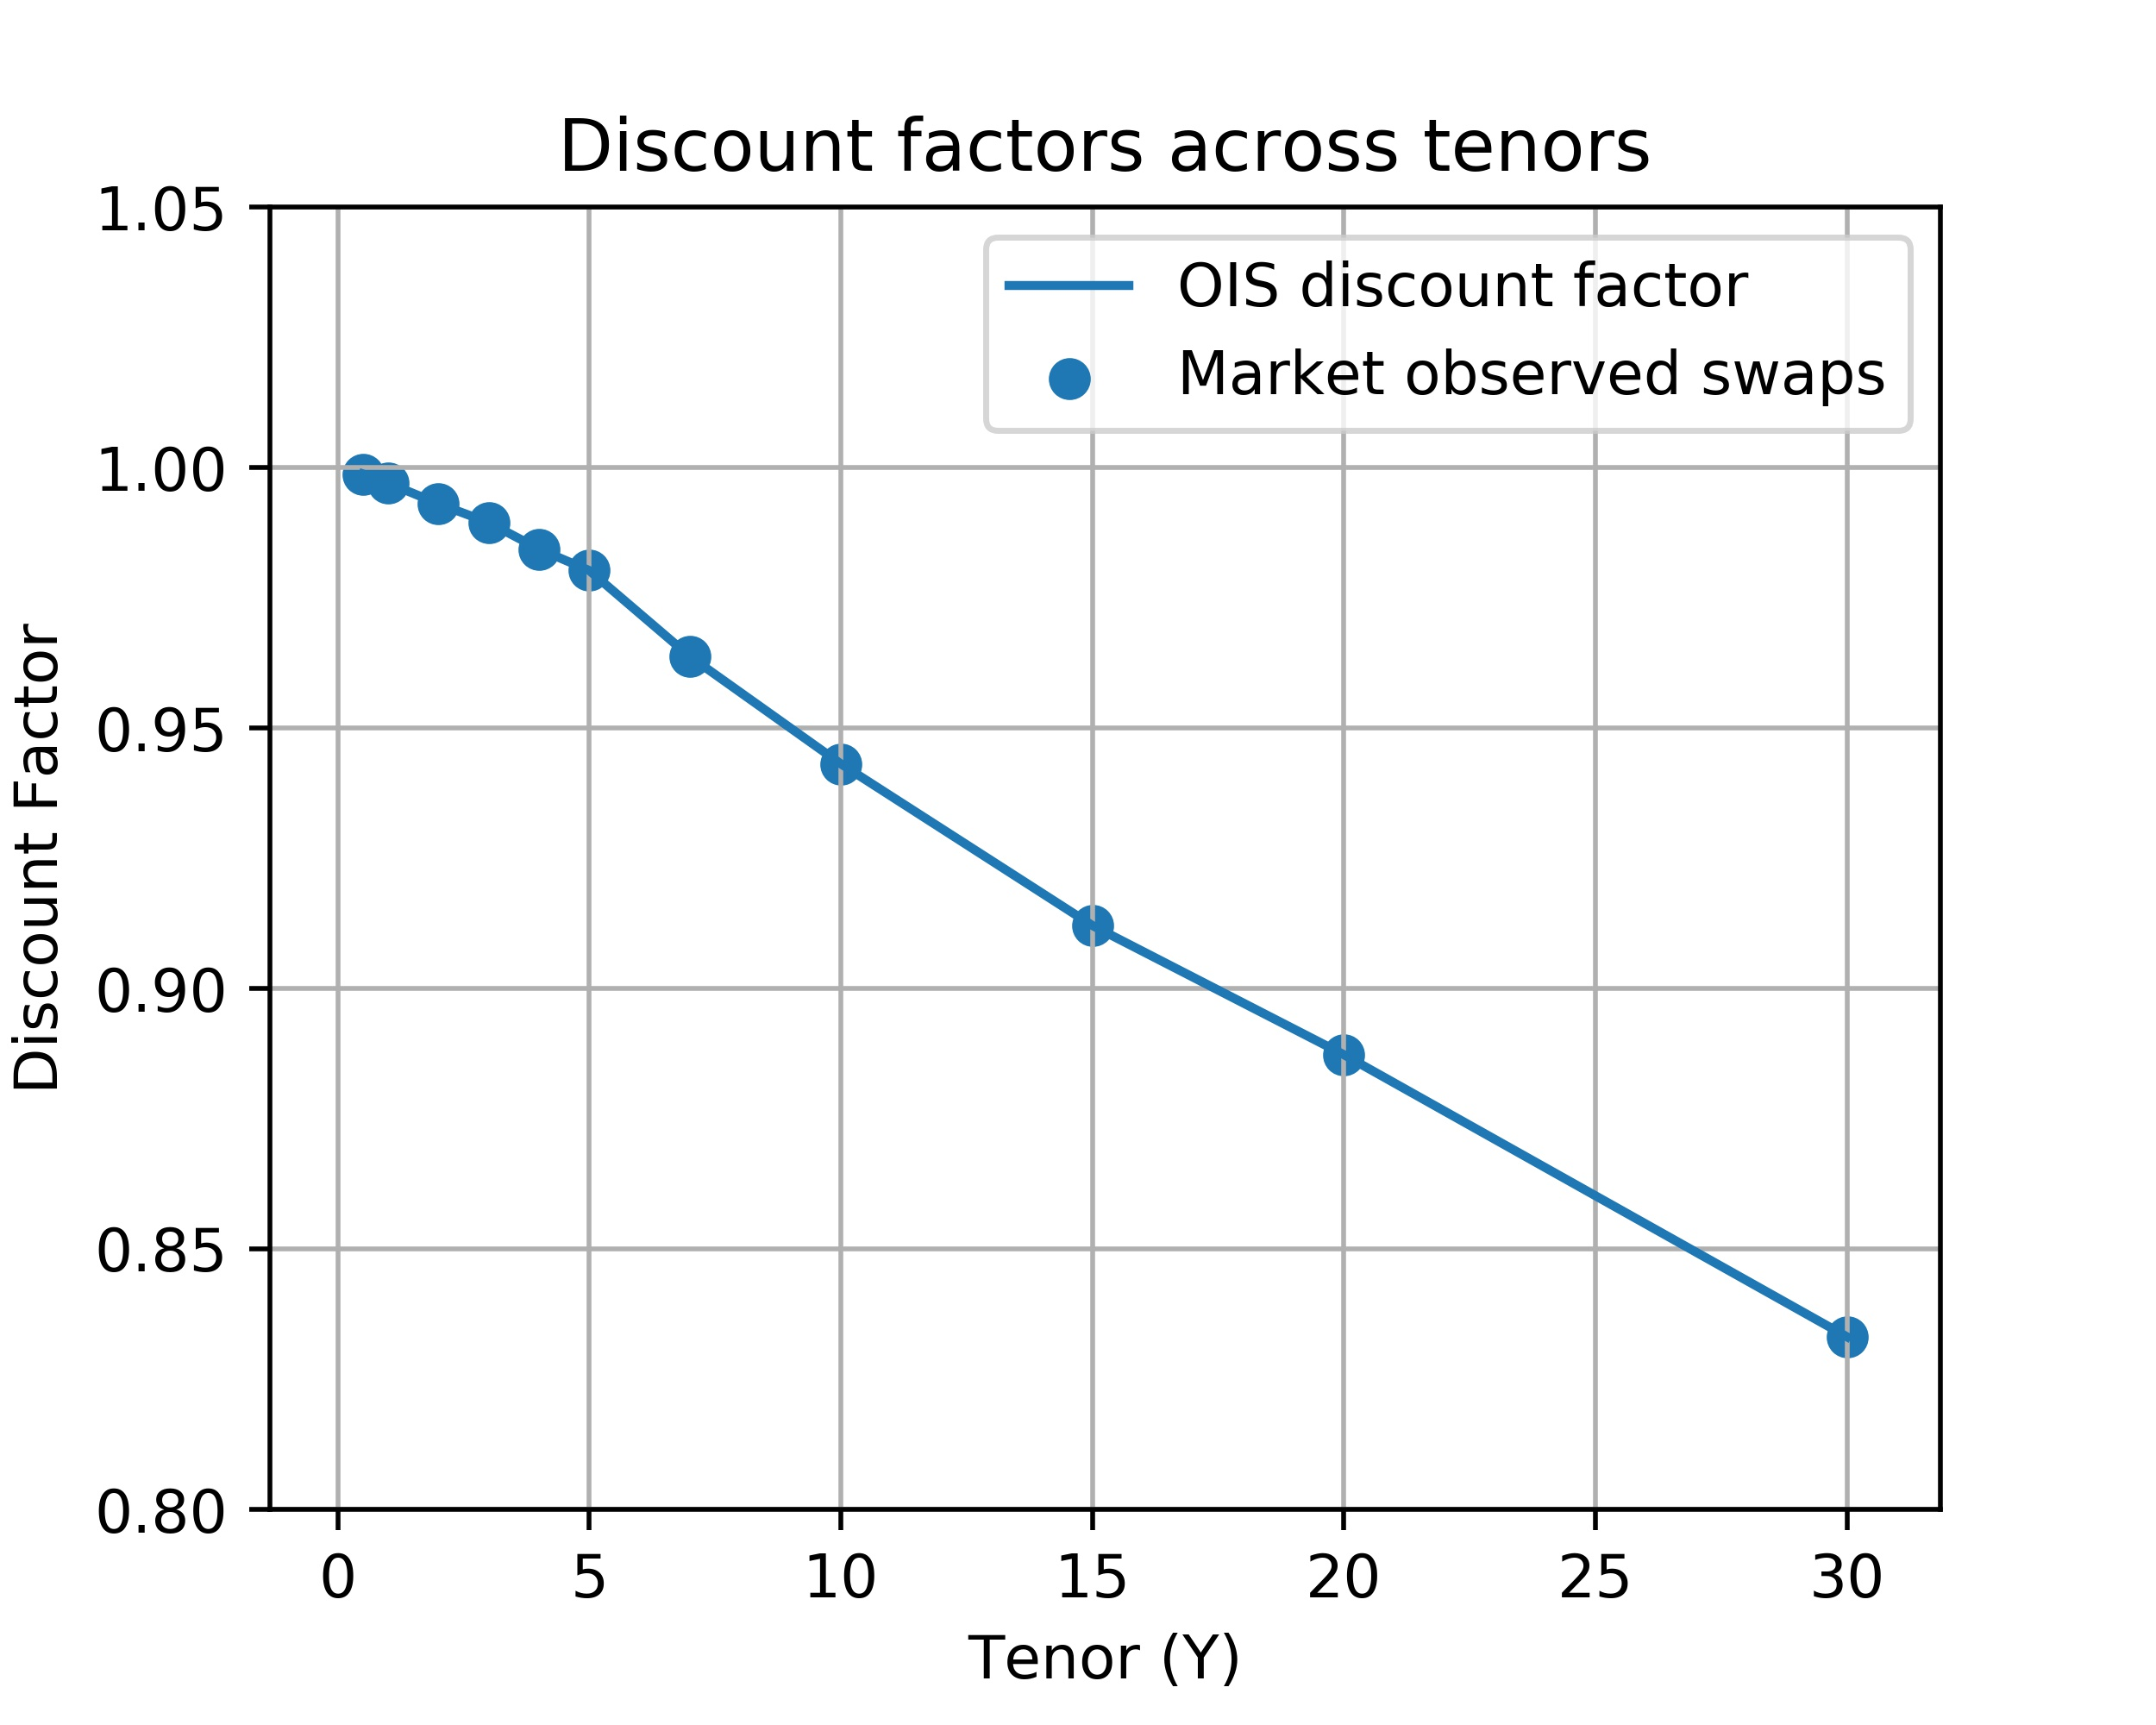
\includegraphics[width=.4\linewidth]{./images/OIS_df.jpg}
		\caption{OIS Discount Curve}
		\label{fig:sub1}
	\end{subfigure}%
	\begin{subfigure}{.5\textwidth}
		\centering
		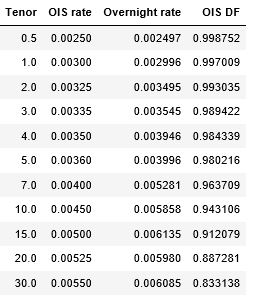
\includegraphics[width=.4\linewidth]{./images/OIStable.jpg}
		\caption{OIS Discount Factors}
		\label{fig:sub2}
	\end{subfigure}
	\caption{OIS Results}
	\label{fig:test}
\end{figure}

\section{LIBOR Discount Factors}

\noindent Similarly for LIBOR discount factors, we will adopt the same approach using the OIS discount factors to derive with the forward libor rates and LIBOR discount factors.

\begin{align*}
PV_{fix} &= PV_{float} \\
0.5 * [D_{OIS}(0,0.5y) + D_{OIS}(0,1y) ] * IRS_{1y} &= 0.5 * [D_{OIS}(0,6m)*L(0,6m)+D_{OIS}(0,1y)*L(6m,1y)] \\
&\vdots \\
0.5 *[D_{OIS}(0,0.5y) + \dots + D_{OIS}(0,20y)] * IRS_{20y} &= 0.5 * [D_{OIS}(0,0.5y) * L(0,6m) + \dots + D_{OIS}(0,20y) * L(19.5y,20y)]
\end{align*} 

\noindent Likewise, we will also substitute the following equations to solve for one unknown (ie. LIBOR discount factor) for each of the above equation starting from 0.5y\dots20y.In this example, we will use 7 years IRS to be consistent with our OIS approach

\begin{align*}
D(0,5.5y) &= \frac{[D(0,7y) - D(0,5y)]}{4} * 1 + D(0,5y) * 2\\
D(0,6y) &= \frac{[D(0,7y) - D(0,5y)]}{4} * 2 + D(0,5y) * 2\\
D(0,6.5y) &= \frac{[D(0,7y) - D(0,5y)]}{4} * 3 + D(0,5y) * 2\\
L(5y,5.5y) &= \frac{D(0,5y) - D(0,5.5y)}{D(0,5.5y)}    \\
L(5.5y,6y) &= \frac{D(0,5.5y) - D(0,6y)}{D(0,6y)}    \\
L(6y,6.5y) &= \frac{D(0,6y) - D(0,6.5y)}{D(0,6.5y)}    \\
L(6.5y,7y) &= \frac{D(0,6.5y) - D(0,7y)}{D(0,7y)}    \\
\end{align*}


\noindent Proceeding to execute the same approach for all IRS , we derive the following LIBOR discount factors results and graph.

\begin{figure}[h]
	\centering
	\begin{subfigure}{.5\textwidth}
		\centering
		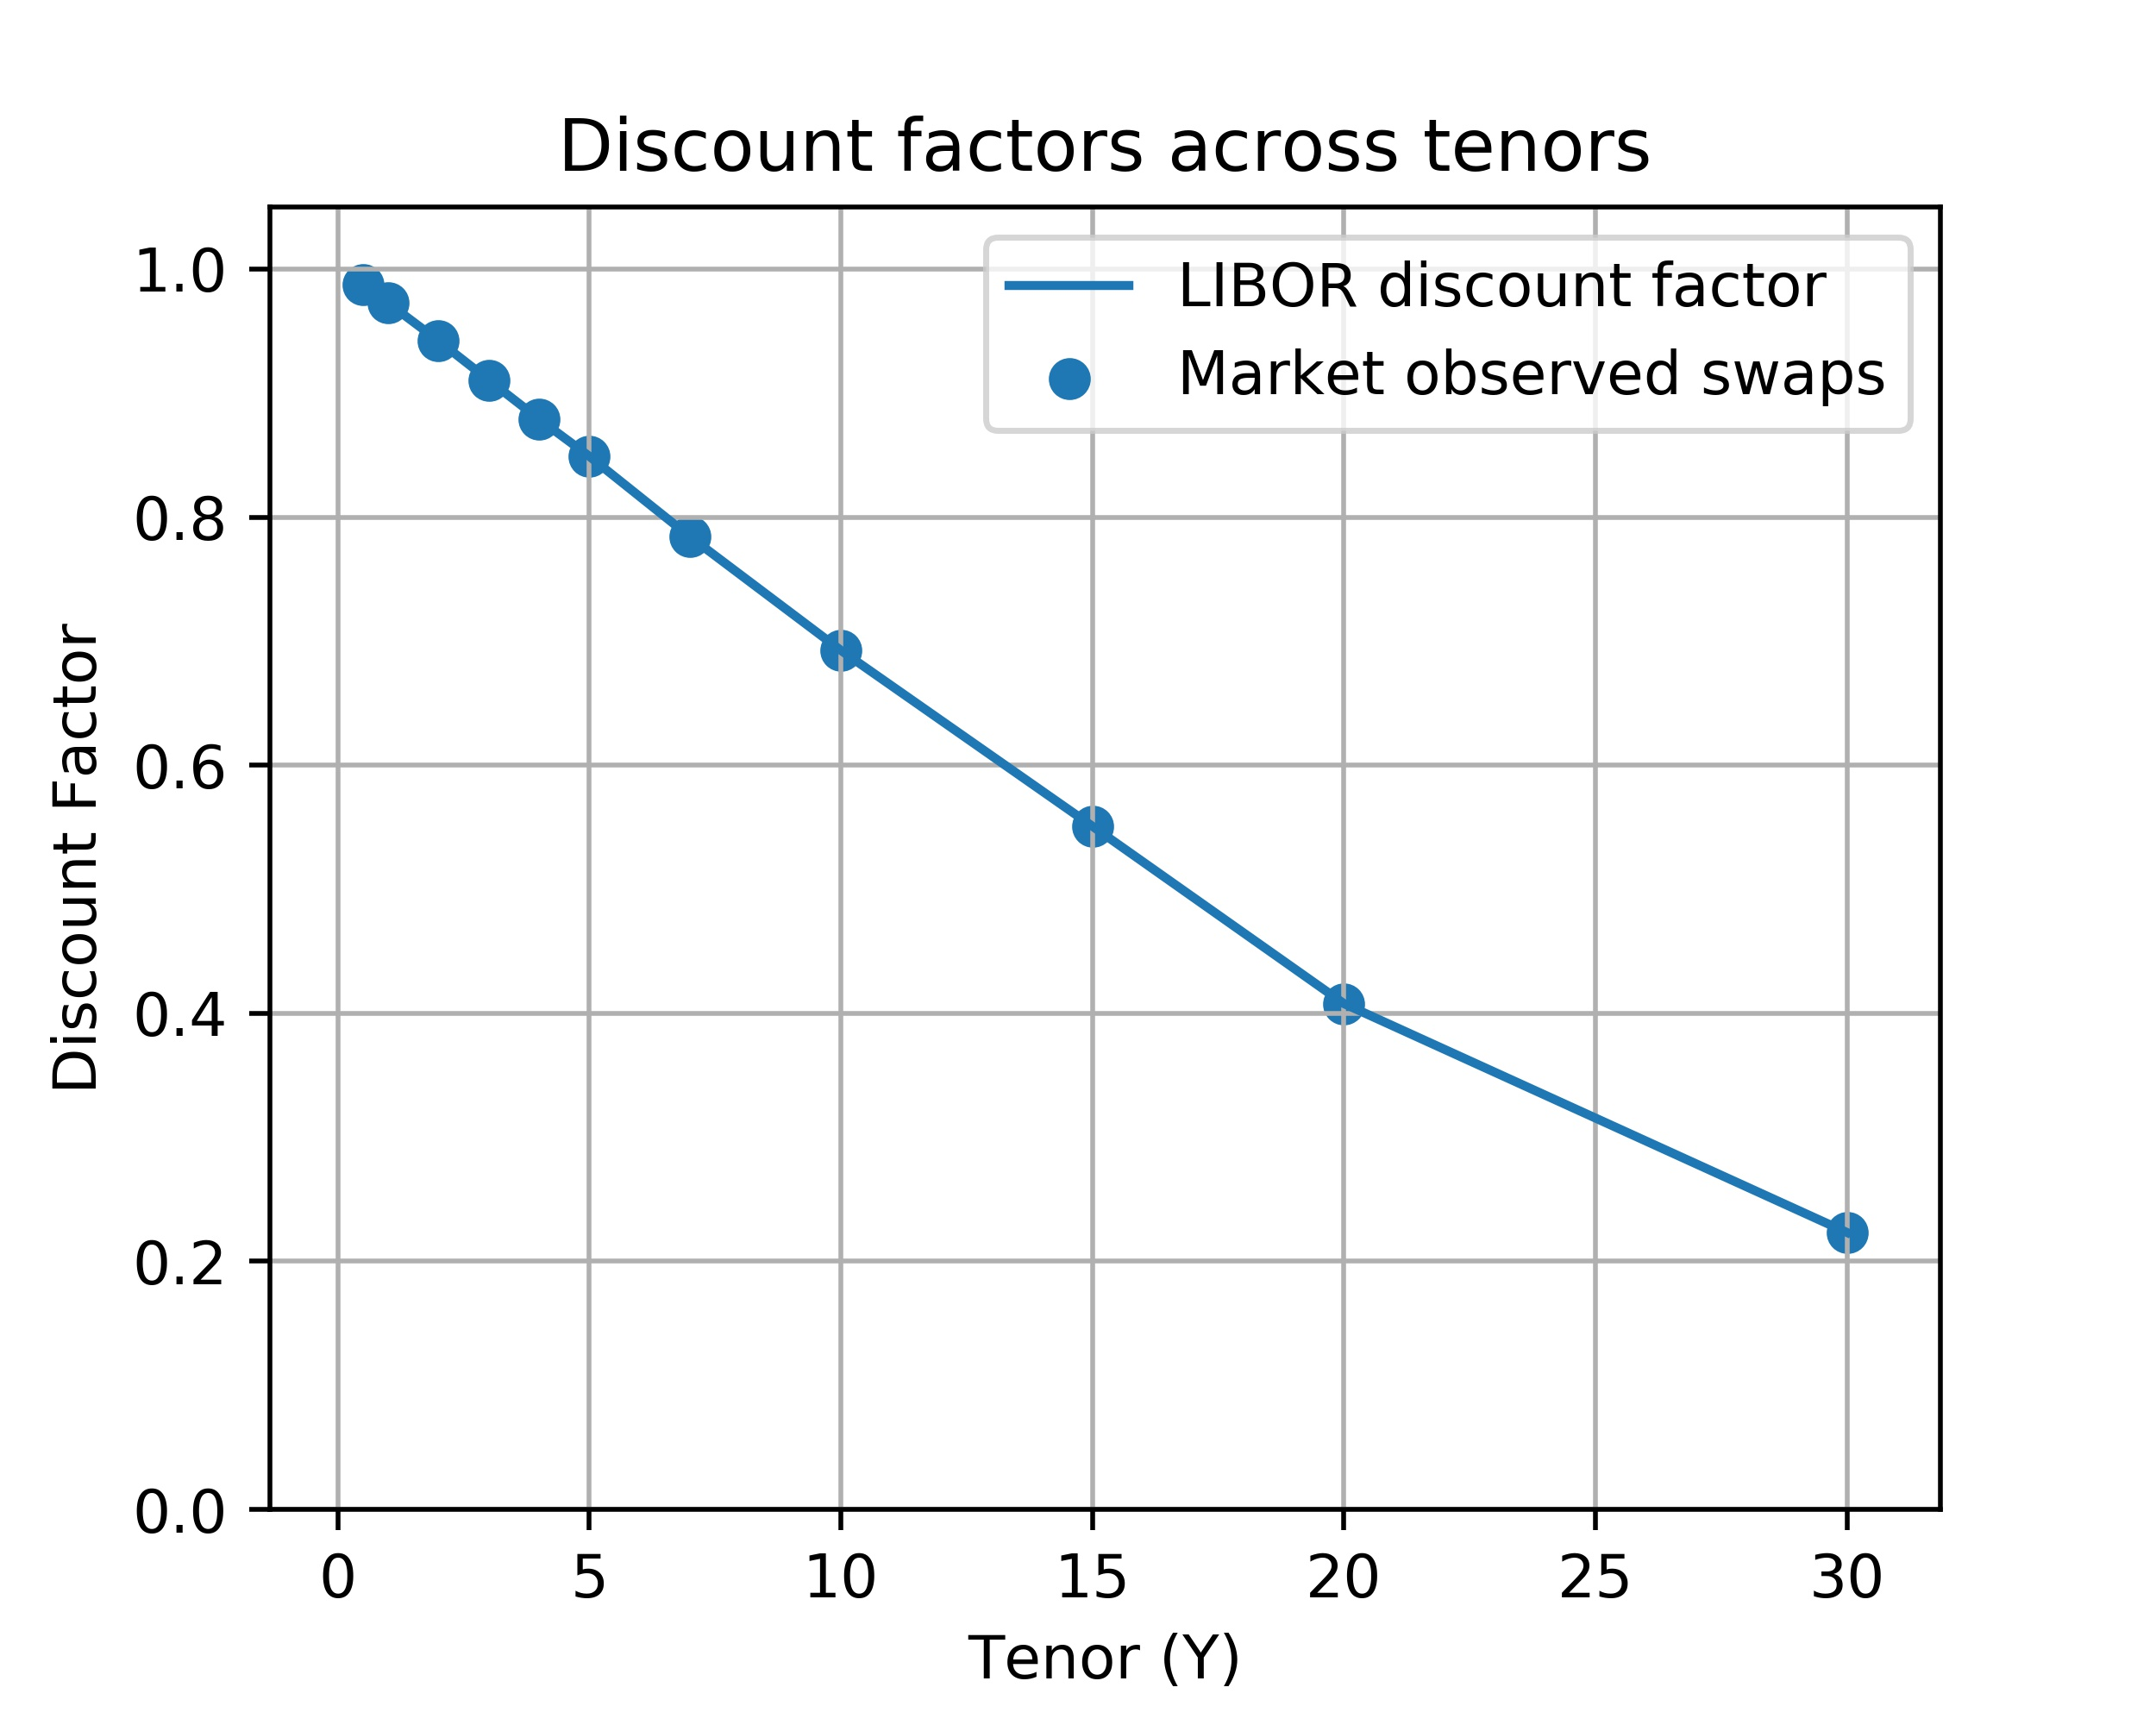
\includegraphics[width=.4\linewidth]{./images/LIBOR_df.jpg}
		\caption{LIBOR Discount Curve}
		\label{fig:sub1}
	\end{subfigure}%
	\begin{subfigure}{.5\textwidth}
		\centering
		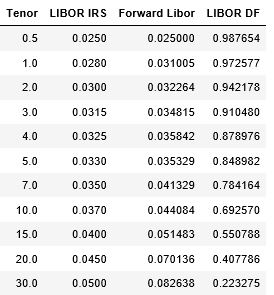
\includegraphics[width=.4\linewidth]{./images/LIBORtable.jpg}
		\caption{LIBOR Discount Factors}
		\label{fig:sub2}
	\end{subfigure}
	\caption{LIBOR Results}
	\label{fig:test}
\end{figure}


\section{Forward Swap Rates}

\noindent With all the necessary OIS discount factors and Forward LIBOR rates, we can go on to derive the Forward Swap rates:

\begin{figure}[ht]
	\centering
	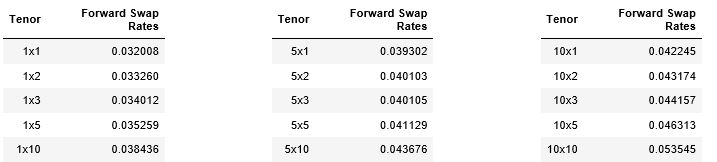
\includegraphics[width= \linewidth]{./images/FwdSwaps.jpg}
	\caption{Forward Swap rates}
\end{figure}


\end{document}